\documentclass[10pt, graphics, aspectratio=169, table]{beamer}
\usepackage{hyperref}
\usepackage{booktabs}
\usepackage{qrcode}
\usepackage[normalem]{ulem}

% -- Change to this year's color! --
\definecolor{ese}{RGB}{58, 240, 212}
\newcommand{\ra}{$\Rightarrow$\ }

\usetheme{metropolis}
\setbeamercolor{frametitle}{bg=ese}

\title{Licenses - Open source}
\author{Eric Wolf}
\date{ESE \the\year{}}
\institute{Nerd::101 - ESE - ifsr - TU Dresden}
\titlegraphic{\hfill
\includegraphics[height=2cm]{../logo}}

\begin{document}
    \maketitle

    \begin{frame}{Outline}
        \tableofcontents
    \end{frame}

    \section{License basics}
    \begin{frame}{What is a license}
        \begin{columns}
            \column{0.55\textwidth}
                \begin{itemize}
                    \item permits you to use or do something
                    \item can contain conditions and limitations
                    \item important when programming professionally
                \end{itemize}
            \column{0.45\textwidth}
                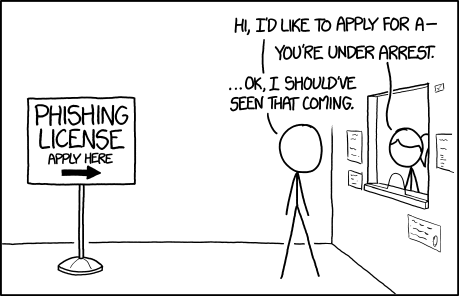
\includegraphics[width=\textwidth]{img/phishing_license.png}
                \center\tiny\url{https://xkcd.com/1694}
        \end{columns}
    \end{frame}

    \begin{frame}{Why are licenses important}
        \begin{itemize}
            \item disobeying a license might lead to criminal charges
            \item publishing your work without a license might prevent others from using it
        \end{itemize}
        \textbf{Using commonly used licenses prevents legal pitfalls}
    \end{frame}

    \begin{frame}{How to apply a license}
        \begin{columns}
            \column{0.55\textwidth}
                \begin{itemize}
                    \item users must be informed about the license
                    \item most projects contain a file called \textbf{LICENSE}
                    \item source files should contain short notices or \href{https://spdx.dev/learn/handling-license-info}{SPDX License Identifiers}
                \end{itemize}
            \column{0.45\textwidth}
                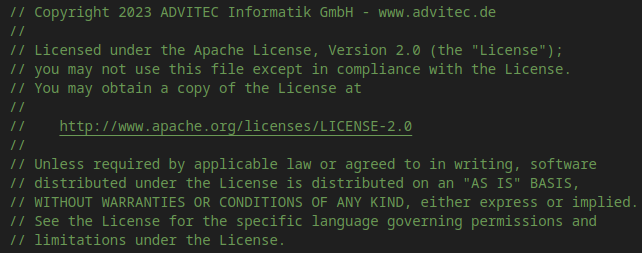
\includegraphics[width=\textwidth]{img/notice_example.png}
                \center\tiny Example of a license notice
        \end{columns}
    \end{frame}


    \section{Permissive licenses}
    \begin{frame}{MIT License}
        \begin{columns}
            \column{0.55\textwidth}
                \begin{itemize}
                    \item allows almost anything, including commercial use and relicensing
                    \item requires copies to include a copyright and permission notice
                    \item does not provide any warranty or liability
                \end{itemize}
                \textbf{Simple license for simple programs}
            \column{0.45\textwidth}
                
\includegraphics[width=\textwidth]{img/MIT.png}
                \center\tiny\href{https://en.m.wikipedia.org/wiki/File:MIT_logo.svg}{MIT Logo}
        \end{columns}
    \end{frame}

    \begin{frame}{Apache License 2.0}
        \begin{columns}
            \column{0.55\textwidth}
                \begin{itemize}
                    \item allows almost anything, like the MIT license
                    \item requires copies to include a copyright and permission notice
                    \item does not provide any warranty or liability
                    \item requires the declaration of changes
                    \item forces contributors to grant patent rights
                    \item expressly does not grant any trademark rights
                \end{itemize}
                \textbf{License aimed at professional open source software}
            \column{0.45\textwidth}
                
\includegraphics[width=\textwidth]{img/Apache.png}
                \center\tiny\href{https://commons.wikimedia.org/wiki/File:ASF_Logo.svg}{Apache Software Foundation Logo}
        \end{columns}
    \end{frame}

    \section{Copyleft licenses}
    \begin{frame}{GNU General Public License}
        \begin{columns}
            \column{0.55\textwidth}
                \begin{itemize}
                    \item enforces the four freedoms (use, study, share, improve)
                    \item requires copies to include a copyright and permission notice
                    \item does not provide any warranty or liability
                    \item forces contributors to grant patent rights
                    \item requires the source code to be disclosed on distribution and the declaration of changes
                    \item requires modifications and larger works to be released under a compatible license
                \end{itemize}
                \textbf{License aimed at free open source software which respects the freedom of its users}
            \column{0.45\textwidth}
                
\includegraphics[width=\textwidth]{img/GPL.png}
                \center\tiny\href{https://commons.wikimedia.org/wiki/File:GPLv3_Logo.svg}{GNU General Public License Logo}
        \end{columns}
    \end{frame}

    \begin{frame}{GNU Lesser General Public License}
        \begin{columns}
            \column{0.55\textwidth}
                \begin{itemize}
                    \item Version of the GPL aimed at libraries
                    \item allows larger works using interfaces provided by the licensed work to use a different license
                    \item requires larger works to allow the licenced work to be replaced and changed
                \end{itemize}
                \textbf{License aimed at free open source libraries which should be useable by proprietary code}
            \column{0.45\textwidth}
                
\includegraphics[width=\textwidth]{img/LGPL.png}
                \center\tiny\href{https://commons.wikimedia.org/wiki/File:LGPLv3_Logo.svg}{GNU Lesser General Public License Logo}
        \end{columns}
    \end{frame}

    \begin{frame}{GNU Affero General Public License}
        \begin{columns}
            \column{0.55\textwidth}
                \begin{itemize}
                    \item Version of the GPL aimed at server software
                    \item requires interaction with the licensed work over the network to be treated as distribution
                    \item prevents application service providers from not having to disclose the source code
                \end{itemize}
                \textbf{License aimed at free open source software which requires additional protection}
            \column{0.45\textwidth}
                
\includegraphics[width=\textwidth]{img/AGPL.png}
                \center\tiny\href{https://commons.wikimedia.org/wiki/File:AGPLv3_Logo.svg}{GNU Affero General Public License Logo}
        \end{columns}
    \end{frame}


    \section{What to do next}
    \begin{frame}{Choose a license}
        \center\qrcode[height=1in]{https://choosealicense.com}
        \center\url{https://choosealicense.com}
    \end{frame}
    
\end{document}